% !Mode:: "TeX:UTF-8"
% !TEX root = ..\Literature_Translation.tex
\kchapter{计算结果}
使用建模语言GAMS(v23.0)建立该数学模型,并用CPLEX 11.2.1.0 使用4核求解。计算实验在一台处理器为Intel i7(2.8GHz, 12GB)的PC 机上运行,所有示例实验时间设为10 h。

这些示例包括15个活动,通常这些活动在工作台上的操作时间要长于夹具。
为了保护公司数据的隐私性,持续时间的单位(t.u.)不表示实际时间,因为其乘上了一个常数。需要注意的是,每架飞机需要两整套装配子集,因此,活动数目被扩大成30个活动。
\begin{table}[h]
  \centering
  \caption{研究示例输入数据}
    \begin{tabular}{ccccccc}
    \toprule
子集 &子集的零件 &活动($j$) &\multicolumn{1}{m{23mm}}{\centering 夹具中的工作站} &\multicolumn{1}{m{23mm}}{\centering 夹具中的持续时间($m_j$)} &  \multicolumn{1}{m{23mm}}{\centering 工作台上的持续时间($q_j$)} &  \multicolumn{1}{m{23mm}}{\centering 前继活动($A(j,k)$) }\\
\midrule
    1     & 1     & 1     & 1     & 5     & 7     & - \\
    1     & 1     & 2     & 1     & 4     & 47    & 1 \\
    2     & 1     & 3     & 1     & 5     & 7     & - \\
    2     & 1     & 4     & 1     & 4     & 47    & 3 \\
    1     & 2     & 5     & 2     & 15    & 29    & - \\
    1     & 2     & 6     & 2     & 9     & 71    & 5 \\
    2     & 2     & 7     & 2     & 15    & 29    & - \\
    2     & 2     & 8     & 2     & 9     & 71    & 7 \\
    1     & 3     & 9     & 3     & 11    & 40    & - \\
    2     & 3     & 10    & 3     & 11    & 40    & - \\
    1     & 4     & 11    & 4     & 12    & 40    & - \\
    1     & 4     & 12    & 4     & 6     & 40    & 11 \\
    2     & 4     & 13    & 4     & 12    & 40    & - \\
    2     & 4     & 14    & 4     & 6     & 40    & 13 \\
    1     & 5     & 15    & 5     & 8     & 30    & - \\
    1     & 5     & 16    & 5     & 6     & 40    & 15 \\
    2     & 5     & 17    & 5     & 8     & 30    & - \\
    2     & 5     & 18    & 5     & 6     & 40    & 17 \\
    1     & 6     & 19    & 6     & 12    & 17    & - \\
    1     & 6     & 20    & 6     & 6     & 40    & 19 \\
    2     & 6     & 21    & 6     & 12    & 17    & - \\
    2     & 6     & 22    & 6     & 6     & 40    & 21 \\
    1     & 7     & 23    & 7     & 7     & 12    & - \\
    1     & 7     & 24    & 7     & 7     & 30    & 23 \\
    2     & 7     & 25    & 7     & 7     & 12    & - \\
    2     & 7     & 26    & 7     & 7     & 30    & 25 \\
    1     & 8     & 27    & 8     & 10    & 61    & - \\
    1     & 8     & 28    & 8     & 12    & 66    & 27 \\
    2     & 8     & 29    & 8     & 10    & 61    & - \\
    2     & 8     & 30    & 8     & 12    & 66    & 29 \\
    \bottomrule
    \end{tabular}
  \label{tab:inputdatainstance}
  \end{table}

\reft{tab:inputdatainstance}展示了本研究示例的数据,需要注意的是,由于活动数量加倍,所有在\reft{tab:inputdatainstance}中的数据也都加倍了,例如持续时间。
前3列确定了子集、零件编号及货都编号,第4列显示了活动($j$)运行的工作站,后面两列参考活动在工作台和夹具的持续时间。最后1列显示了活动$j$的前继活动。

\reft{tab:inputdatainstance}所示的第1个实验集合用到了阶段1的模型求解,当和其他阶段的模型之解相比较时,其对应为装配2个子集所需最短时间。
由于在实践是会用到最小的生产率,执行项目需要288个时间单位(t.u.),然后假设所有在阶段2,3,4完成的示例都在最短制造期内完成,即在阶段1找到的解和288个时间单位之间。

\ksection{阶段1的结果}
阶段1模型的结果是278个整数变量,310个实数变量,并在0.017\ min 内得解。最短制造期为161\ t.u.,通过13位工人,可见\reff{fig:stage1model}。
\begin{figure}[h]
\begin{floatrow}[2]
\centering
\ffigbox{\caption{阶段1模型求解\label{fig:stage1model}}}{\includegraphics[width = 8cm,height = 4cm]{stage1model.bmp}}
\ffigbox{\caption{阶段2的最佳工人数和制造期}\label{fig:stage2worksandmakespan}}{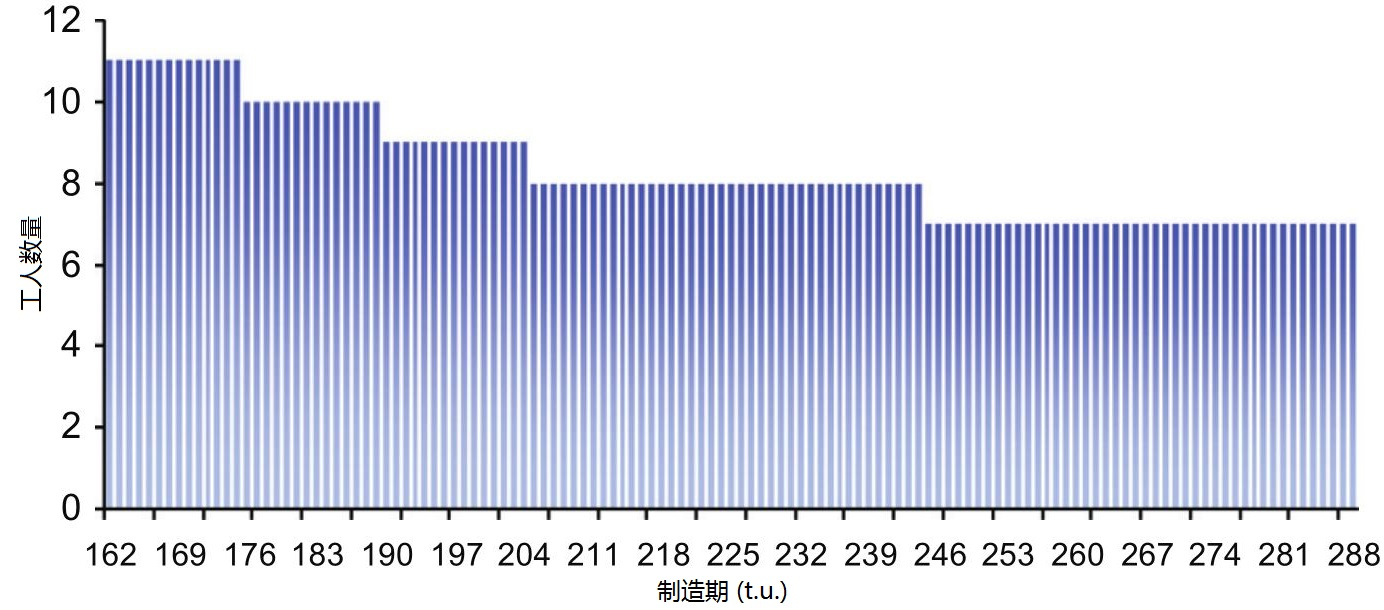
\includegraphics[width=8cm,height = 4cm,trim = 0 -30 0 0 ]{stage2teammakespan.jpg}}
\end{floatrow}
\end{figure}
需要注意的是,这个解没有水平分级,因为目标函数是最小化制造期,而其他阶段的目标函数式最小化工人数。因此,在用阶段2,3,4的模型时,要根据队伍的熟练程度,有可能显示在161\ t.u. 完成所有任务。
在阶段2,工人总数可以从13减少到11。

为了评估阶段2,3,4模型的运行情况,127个示例需要求解,它们的制造期根据\reft{tab:inputdatainstance}变化从161\ t.u. 到288\ t.u.。

\ksection{阶段2模型求解}
在阶段2,零件需要经两队人组装:一队是在装配夹具中操作,另一队人负责在工作台操作。考虑由11位工人负责的最短制造期得到的结果,和由7位工人负责的制造期为288单位时间得到的结果。
\reff{fig:stage2worksandmakespan}说明了阶段2对于每个制造期所需的工人数量。劳动力/制造期权衡曲线说明了不同制造期对队伍规模的影响,是一个离散的水平图形。
这个信息可以用于快速找出适用于所有制造期情形的装配队伍规模,在给定的两个步长间的距离的前提下,即选择某个确定队伍规模的风险,对于分析队伍的反应和能力也是很有用的。
举例来说,在\reff{fig:stage2worksandmakespan}中,选取制造期为188\ t.u.,需要9个工人。
如果在制造过程中的某个变量需要更短的装配时间,即更短的制造期,这样便需要雇佣额外的工人。
然而,若考虑制造期为204\ t.u.,如果需要更短的装配时间,则可能不需要另外雇佣工人,因为制造期只有188\ t.u.。
\begin{figure}[h]
\begin{floatrow}[2]
\centering
\ffigbox{\caption{阶段2各制造期下的计算时间\label{fig:stage2computationalvsmakespan}}}{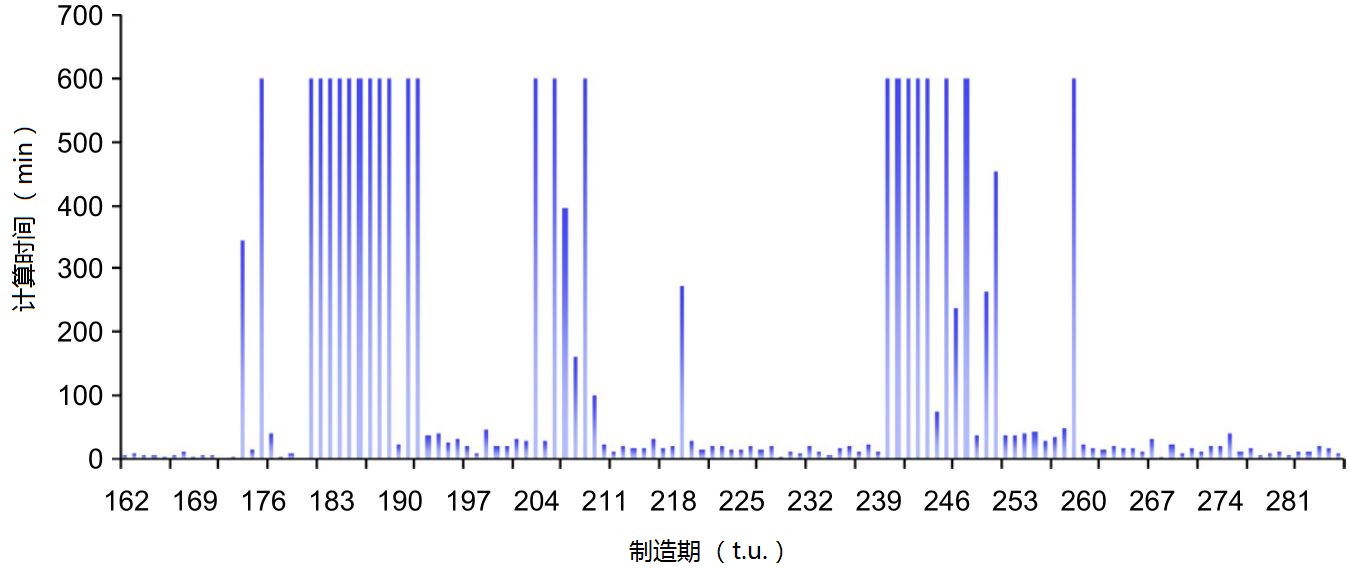
\includegraphics[width = 8cm,height = 4cm]{stage2computationaltimeandmakespan}}
\ffigbox{\caption{阶段3的队伍规模和制造期}\label{fig:stage3worksvsmakespan}}{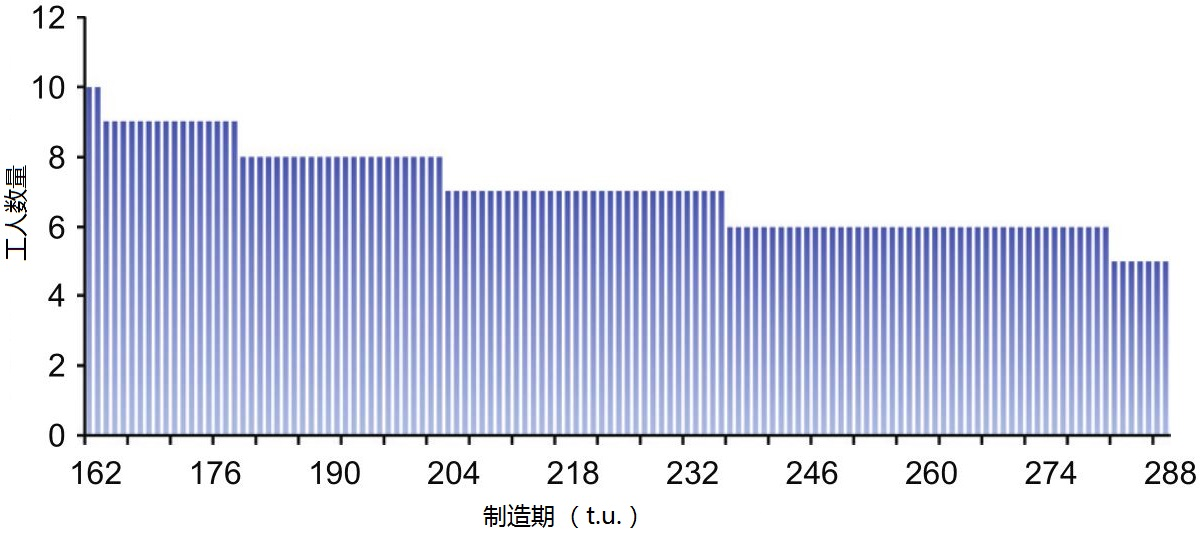
\includegraphics[width=8cm,height = 4cm]{stage3worksvsmakespan}}
\end{floatrow}
\end{figure}

\reff{fig:stage2computationalvsmakespan}展示了为得到\reff{fig:stage2worksandmakespan}结果花费的计算时间。
需要注意,虽然有些示例达到了最大计算限制600\ min,大多数时在前100\ min 内完成的,可能通过已知的示例最优解检验,以得到该示例的上下界,对应于小于和大于现行示例的制造期。
显然,如果下界或上界有着同样的最优值,即它们需要的工人数一样,那么这个便是示例的最优解。

\ksection{阶段3模型求解}
在阶段3需要考虑两队人,第1个队伍是由专业工人组成的,可以在装配夹具和工作台操作,另一队人由非专业工人组成,只能在工作台操作。因此,我们期望在对比阶段2和阶段3时,对于同样的制造期,可以得到更少的工人量。
例如,考虑制造期为162\ t.u.的例子,阶段2需要11个工人,而阶段3只要10个。\reff{fig:stage3worksvsmakespan}显示了模型\eqref{equb:19} -- (\ref{equb:26})的求解结果。
\begin{figure}[h]
\centering\caption{阶段3用\eqref{equb:19} -- (\ref{equb:26})得到的各制造期计算时间\label{fig:stage3computationalvsmakespan}}
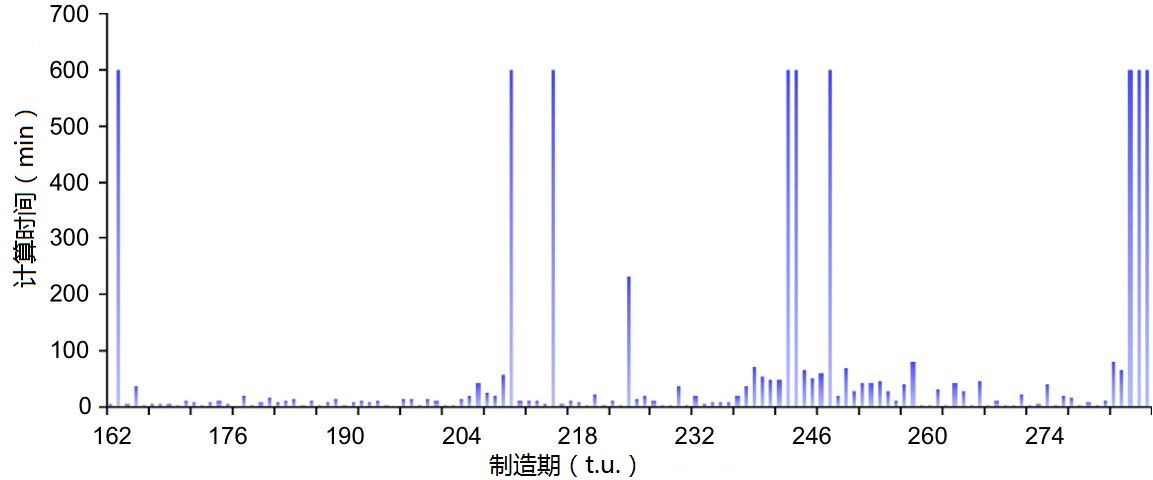
\includegraphics[width = 12cm]{stage3computvsmakespan}
\end{figure}

\reff{fig:stage3computationalvsmakespan}展示了用\eqref{equb:19} -- (\ref{equb:26})的求解结果得到的计算时间。
需要注意的是,有许多示例达到了容许的最大计算时间限制,但大多数示例的求解时间少于100,即只要少数达到了最大计算时间限制。

\ksection{阶段4模型求解}
在阶段4,所有工人都可以在夹具和工作台上操作。因此,阶段3的结果可作为阶段4结果的上界。
\begin{figure}[h]
\begin{floatrow}[2]
\centering
\ffigbox{\caption{阶段4模型下最优工人数量规模与其制造期\label{fig:stage4workersvsmakespan}}}{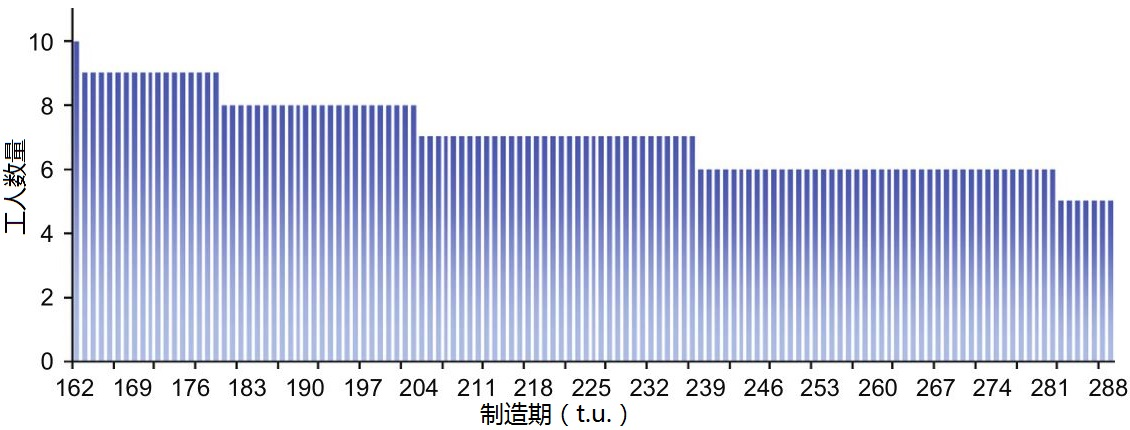
\includegraphics[width = 8cm,height = 4cm]{stage4optteamsizevsmakespan}}
\ffigbox{\caption{阶段4通过模型得到的各制造期计算时间}\label{fig:stage4computimevsmakespan}}{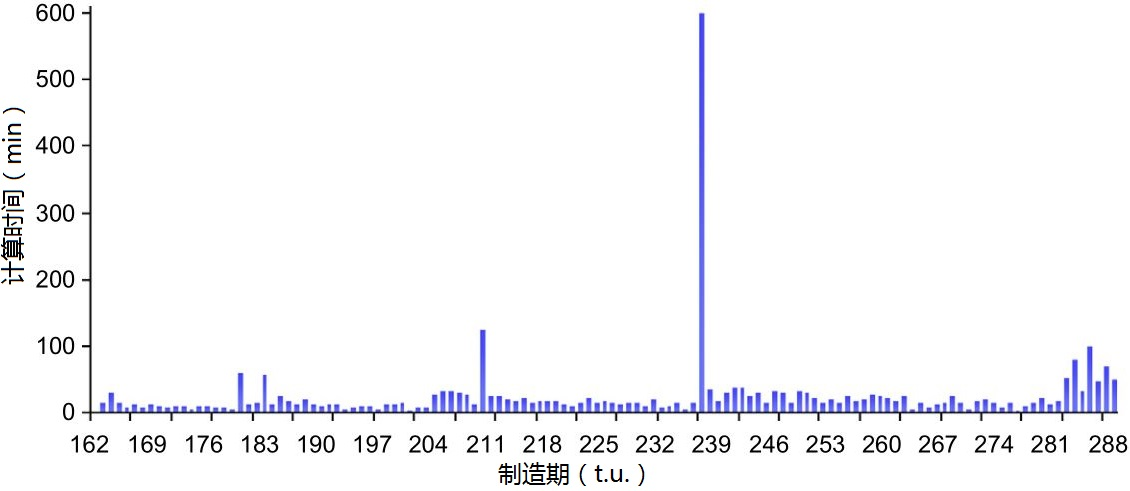
\includegraphics[width=8cm,height = 4cm]{stage4compuvsmakespan}}
\end{floatrow}
\end{figure}
\reff{fig:stage4workersvsmakespan}说明了阶段4的人工曲线。例如制造期为162\ t.u.,阶段4需要10位给人,和阶段3一样。
除了制造期为163\ t.u.,阶段4可以找到比阶段3更优的解,其他的人工数皆未减少。\reff{fig:stage4computimevsmakespan}显示了找到阶段4的结果的计算时间。
\begin{figure}[h]
\centering\caption{阶段4制造期为288\ t.u.的生产调度Gantt 图\label{fig:stage4gantt288}}
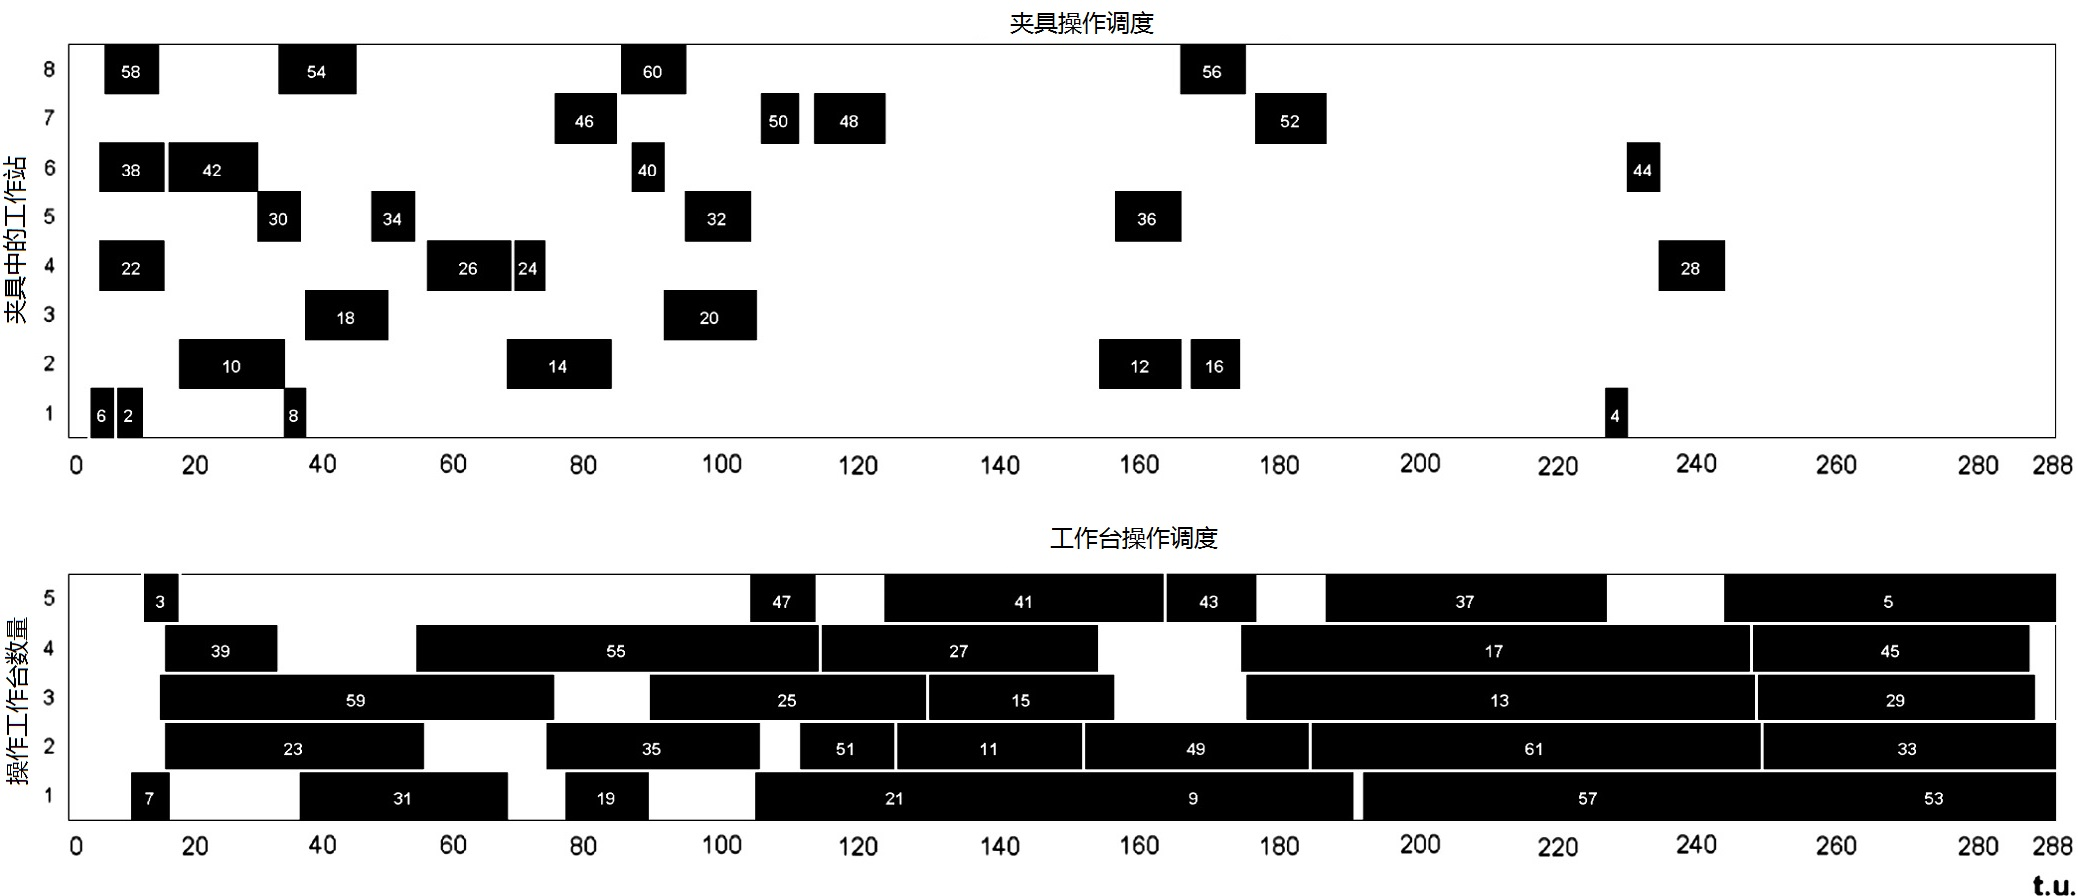
\includegraphics[width = 15cm]{288gantt}
\end{figure}

\reff{fig:stage4gantt288}展示了一个制造期为288\ t.u.的调度的例子。注意到,Gantt 图说明了夹具的调度存在空白区域,对应于夹具中工作站为空闲的时域,这是邻接约束造成的。

\reft{tab:inputdatainstance}中,装配飞机有有30个活动。考虑到每个活动有两个操作,一个在夹具上,一个在工作台上。
这样的话,在\reft{tab:inputdatainstance}中的活动可以看作\reff{fig:stage4gantt288}中的操作2和3,活动2对应于操作4,5,以此类推。
因此,总操作数为62,包括30个在夹具中的操作,30个在工作台的操作,2个人工/虚构操作1和62。

在工作车间,工厂用8位工人于制造期为288生产,然而找到如\reff{fig:stage3worksvsmakespan}所示的解,说明所有工作有可能只用5位工人就可按时完成,即少了37\% 的人工。


\kchapter{总结}
我们在本文研究了在航空工厂内有邻接约束的生产调度问题。4种主要的人员学习/熟练阶段在装配过程中产生,我们分析并提出了各阶段的混合整数线性规划模型。
这些模型通过优化软件GAMS/CPLEX 搭建,并在可接受的计算运行时间内求解。
所得的数值结果和实际数据进行了对比,用模型求解的结果所需工人数要比原有的工厂人数少37\%。

各阶段生成了劳动力权衡曲线,这些曲线在生产计划改变时很有实用价值,可以给生产管理员提供快速响应策略。
这些信息也有助于使偶然计划变得详尽,由于这些信息显示了有可调配的人员数量。

调查其他解决此问题的方法的研究是有意义的,基于启发式和元启发式方法可以求解这些方法不能在合理计算时间内求解的大型问题。
其他目标函数,例如资源等级,也可以用于此方法。
该研究的另一个有用的拓展是,可在强健随机规划和强健最优化的前提下研究此问题,例如考虑不确定持续时间的装配操作。